\chapter{unused stars}
\label{sec:listing}
\lstset{style=68KStyle}

Tempest 2000 is full of starfields, from the title screen to the game itself - there's always a field of stars up to something in the background.

\begin{figure}[H]
    \centering
    \begin{adjustbox}{width=12cm,center}
      \frame{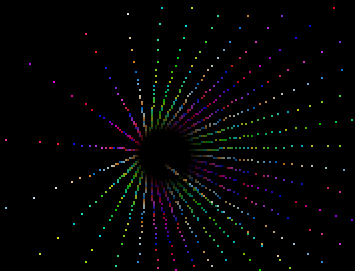
\includegraphics[width=4cm]{src/starfield/ring/starfield11.png}}%
      \hspace{0.5cm}
      \frame{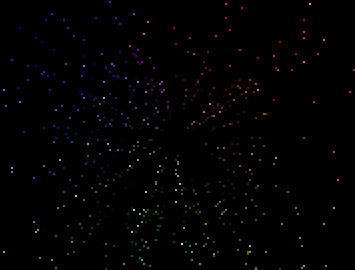
\includegraphics[width=4cm]{src/starfield/unused/unused-starfield-03.png}}%
      \hspace{0.5cm}
      \frame{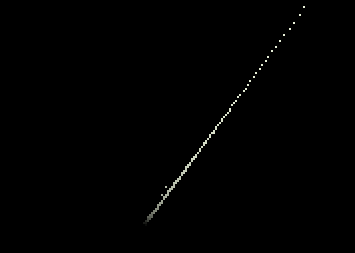
\includegraphics[width=4cm]{src/starfield/ptunnel/ptunnel-starfield-23.png}}%
    \end{adjustbox}
  \caption{Example of starfield effects. The middle one is not used by the game.}
\end{figure}

We'll start in totally the wrong place by looking at piece of code that actually goes unused in the game. A routine called
\icode{initstarfield} that populates a random space of stars. This was probably a first iteration at drawing a star-spangled
background and dropped later when fancier alternatives were developed. Before we look at the fancy, and necessarily more complex
alternatives, let's take a look at what populating a random-ish starfield looks like.

What we have to do first is populate a data structure for our starfield. This is a list (or array) of elements with each element containing an X, Y,
and Z co-ordinate plus a color value for the star. There are 127 such elements in total, and we store the number of elements as a 'header' or first entry
in the array. We'll store this array in an address called \icode{field1} and do the work of populating it in a routine called \icode{initstarfield}.

The values we come up with for X and Y are totally random. All we do is come up with a number between
0 and 127 for the X and Y co-ordinates and a number between 0 and 512 for our Z co-ordinate. We then use the X and Y co-ordinates
to seed a color value.

Here is the routine. As we said before, it ended up unused but has the merit of being relatively simple to read and understand:
\begin{lstlisting}[caption=Populating an unused starfield data structure. This is a fuzzier version of the ring starfield used in the credits screen.]
initstarfield:
;
; initialise a starfield data structure for the GPU to display

  lea field1,a0     ; field1 is where the data structure is stored
  move #127,d7      ; The number of times to loop through 'isf' below.
  move.l #128,(a0)+ ; Store the number of stars at the start of field1.
  ; Create 128 stars and store them as an array in field1.
  ; Each star is: X,Y,Z,cry_index
isf:
  bsr rannum      ; Get a random number between 0 and 255 and store in d0
  move d0,d2      ; Stow d0 in d2 for use later
  sub #$80,d0     ; Get rid of the high bit so the num is between 0 and 128
  swap d0         ; Turn e.g. 00000032 into 00320000
  move.l d0,(a0)+ ; Store our rand num as our X co-ordinate.

  bsr rannum      ; Get a random number between 0 and 255  and store in d0
  move d0,d3      ; Stow d0 in d3 for use later
  sub #$80,d0     ; Get rid of the high bit so the num is between 0 and 128
  swap d0         ; Turn e.g. 00000032 into 00320000
  move.l d0,(a0)+ ; Store our rand num as our Y co-ordinate.

  bsr rannum      ; Get a random number between 0 and 255  and store in d0
  asl #1,d0       ; Multiply the number by 2 so that its between 0 and 512
  swap d0         ; Turn e.g. 00000032 into 00320000
  move.l d0,(a0)+ ; Store our rand num as our Z co-ordinate.

  ; Use our X and Y co-ordinates to come up with a random color for the star.
  ; So if X(d2) is 00000032 and Y(d3) is 00000088:
  and #$f0,d2  ; 00000032 -> 00000030
  lsr #4,d3    ; 00000088 -> 80000008
  and #$0f,d3  ; 80000008 -> 00000008
  or d2,d3     ; 00000030 or 00000008 -> 00000038
  lsl #8,d3    ; 00000038 -> 00003800
  move d3,(a0) ; Store our color value.

  lea 20(a0),a0  ; Move a0 20 bytes ahead ready for the next element.
  dbra d7,isf    ; Loop until d7 is 0.
  rts
\end{lstlisting}

This is our data structure (or at least the first 2 elements in it) in a table:

\begin{figure}[H]
  {
    \setlength{\tabcolsep}{3.0pt}
    \setlength\cmidrulewidth{\heavyrulewidth} % Make cmidrule = 
    \begin{adjustbox}{width=7cm,center}

      \begin{tabular}{lllll}
        \toprule
        Value & Decimal & Description\\
        \midrule
        \icode{0000000E} & 127 & Number of Elements\\
        \icode{00064000} & 127 & Element 1: X co-ordinate\\
        \icode{00064000} & 127 & Element 1: Y co-ordinate\\
        \icode{00064000} & 127 & Element 1: Z co-ordinate\\
        \icode{00064000} & 127 & Element 1: Color Value\\
        \icode{00064000} & 127 & Element 2: X co-ordinate\\
        \icode{00064000} & 127 & Element 2: Y co-ordinate\\
        \icode{00064000} & 127 & Element 2: Z co-ordinate\\
        \icode{00064000} & 127 & Element 2: Color Value\\
        \bottomrule
      \end{tabular}
    \end{adjustbox}
  }\caption*{First 2 elements of the data structure created by \icode{initstarfield}.}
\end{figure}

And this is what our data structure looks like when its animated by our shader \icode{fastvector} (more of which later).

\begin{figure}[H]
    \centering
    \begin{adjustbox}{width=12cm,center}
      \frame{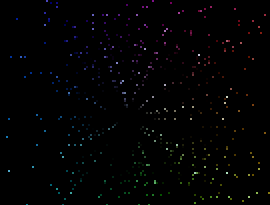
\includegraphics[width=6cm]{src/starfield/unused/unused-starfield-01.png}}%
      \hspace{0.5cm}
      \frame{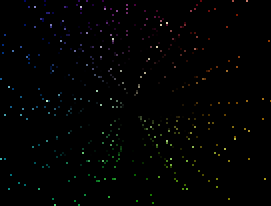
\includegraphics[width=6cm]{src/starfield/unused/unused-starfield-02.png}}%
    \end{adjustbox}
  \caption{Frames of the unused starfield during animation.}
\end{figure}

The actual starfield used in the credits screen makes use of a sine table to accurately calculate the co-ordinates
of pixels in an expanding ring structure.

\begin{lstlisting}
sines:
dc.w $0003,$0609,$0C0F,$1215,$181B,$1E21,$2427,$2A2D
dc.w $3033,$3639,$3B3E,$4144,$4649,$4B4E,$5053,$5557
dc.w $595C,$5E60,$6264,$6667,$696B,$6D6E,$7071,$7274
dc.w $7576,$7778,$797A,$7B7B,$7C7D,$7D7E,$7E7E,$7E7E
dc.w $7E7E,$7E7E,$7E7E,$7D7D,$7C7B,$7B7A,$7978,$7776
dc.w $7573,$7271,$6F6E,$6C6B,$6967,$6563,$615F,$5D5B
dc.w $5957,$5552,$504D,$4B48,$4643,$403E,$3B38,$3533
dc.w $302D,$2A27,$2421,$1E1B,$1815,$120F,$0C08,$0502
dc.w $00FD,$FAF7,$F4F0,$EDEA,$E7E4,$E1DE,$DBD8,$D5D2
dc.w $CFCD,$CAC7,$C4C1,$BFBC,$B9B7,$B4B2,$B0AD,$ABA9
dc.w $A6A4,$A2A0,$9E9C,$9A98,$9795,$9392,$908F,$8D8C
dc.w $8B8A,$8988,$8786,$8584,$8483,$8382,$8282,$8282
dc.w $8282,$8282,$8283,$8383,$8485,$8586,$8788,$898A
dc.w $8B8D,$8E8F,$9192,$9496,$9799,$9B9D,$9FA1,$A3A5
dc.w $A7AA,$ACAE,$B1B3,$B6B8,$BBBD,$C0C3,$C5C8,$CBCE
dc.w $D1D4,$D7D9,$DCDF,$E2E6,$E9EC,$EFF2,$F5F8,$FBFE
dc.w $0000,$0192,$0323,$04B5,$0645,$07D5,$0963,$0AF0 
dc.w $0C7C,$0E05,$0F8C,$1111,$1293,$1413,$158F,$1708
dc.w $187D,$19EF,$1B5C,$1CC5,$1E2A,$1F8B,$20E6,$223C
dc.w $238D,$24D9,$261F,$275F,$2899,$29CC,$2AFA,$2C20
dc.w $2D40,$2E59,$2F6B,$3075,$3178,$3273,$3366,$3452
dc.w $3535,$3611,$36E4,$37AE,$3870,$3929,$39DA,$3A81
dc.w $3B1F,$3BB5,$3C41,$3CC4,$3D3D,$3DAD,$3E14,$3E70
dc.w $3EC4,$3F0D,$3F4D,$3F83,$3FB0,$3FD2,$3FEB,$3FFA
dc.w $3FFF,$3FFA,$3FEB,$3FD2,$3FB0,$3F83,$3F4D,$3F0D 
dc.w $3EC4,$3E70,$3E14,$3DAD,$3D3D,$3CC4,$3C41,$3BB5
dc.w $3B1F,$3A81,$39DA,$3929,$3870,$37AE,$36E4,$3611
dc.w $3535,$3452,$3366,$3273,$3178,$3075,$2F6B,$2E59
dc.w $2D40,$2C20,$2AFA,$29CC,$2899,$275F,$261F,$24D9
dc.w $238D,$223C,$20E6,$1F8B,$1E2A,$1CC5,$1B5C,$19EF
dc.w $187D,$1708,$158F,$1413,$1293,$1111,$0F8C,$0E05
dc.w $0C7C,$0AF0,$0963,$07D5,$0645,$04B5,$0323,$0192 ; <-- sine ($0C7C)
dc.w $0000,$FF6E,$FDDD,$FC4B,$FABB,$F92B,$F79D,$F610 
dc.w $F484,$F2FB,$F174,$EFEF,$EE6D,$ECED,$EB71,$E9F8
dc.w $E883,$E711,$E5A4,$E43B,$E2D6,$E175,$E01A,$DEC4
dc.w $DD73,$DC27,$DAE1,$D9A1,$D867,$D734,$D606,$D4E0
dc.w $D3C0,$D2A7,$D195,$D08B,$CF88,$CE8D,$CD9A,$CCAE
dc.w $CBCB,$CAEF,$CA1C,$C952,$C890,$C7D7,$C726,$C67F
dc.w $C5E1,$C54B,$C4BF,$C43C,$C3C3,$C353,$C2EC,$C290
dc.w $C23C,$C1F3,$C1B3,$C17D,$C150,$C12E,$C115,$C106 ; <-- cosine ($C23C)
dc.w $C101,$C106,$C115,$C12E,$C150,$C17D,$C1B3,$C1F3
dc.w $C23C,$C290,$C2EC,$C353,$C3C3,$C43C,$C4BF,$C54B
dc.w $C5E1,$C67F,$C726,$C7D7,$C890,$C952,$CA1C,$CAEF
dc.w $CBCB,$CCAE,$CD9A,$CE8D,$CF88,$D08B,$D195,$D2A7
dc.w $D3C0,$D4E0,$D606,$D734,$D867,$D9A1,$DAE1,$DC27
dc.w $DD73,$DEC4,$E01A,$E175,$E2D6,$E43B,$E5A4,$E711
dc.w $E883,$E9F8,$EB71,$ECED,$EE6D,$EFEF,$F174,$F2FB
dc.w $F484,$F610,$F79D,$F92B,$FABB,$FC4B,$FDDD,$FF6E 
\end{lstlisting}

A table like this allows us to 'hard code' the points of an arbitrarily sized circle by providing the sine and cosine
values for each point. To get the X and Y co-ordinates of a specific point in the circle you pull out the corresponding sine and cosine
values from the table, multiply each by your desired radius, and that gives you your X and Y value to draw your point
on the screen. You do that for each point (say 32 in total) and you have a ring of dots that you can connect to form
a circle.

\begin{equation}
  x = \cos(\theta) * radius
\end{equation}

\begin{equation}
  y = \sin(\theta) * radius
\end{equation}

The \icode{sines} table seems inscrutable at first glance but the specific use of it made by the \icode{ringstars}
routine is straightforward. The routine plots a circle of 32 points and for each point it uses the current point
number (e.g. 31) to pull out a sine and cosine value from the first entry in the corresponding row on the table. 
If we imagine we're plotting the 31st point this means for the sine value, we will take the first value
from row 31, and for the cosine value it will take the first value 8 rows after that.
As you can see in the above table this corresponds to \icode{\$0C7C} for the sine and \icode{\$C23C} for the cosine.

With this in hand, and a radius of 200 pixels, we can calculate our X and Y co-ordinates. The steps are the same for 
both the X and Y values, except for the use of \icode{sine} and \icode{cosine}:

\begin{figure}[H]
  {
    \setlength{\tabcolsep}{3.0pt}
    \setlength\cmidrulewidth{\heavyrulewidth} % Make cmidrule = 
    \begin{adjustbox}{width=9cm,center}

      \begin{tabular}{lllll}
        \toprule
        Step No. & Description & Cosine & Sine\\
        \midrule
        1 & Value taken from \icode{sine} table & \icode{\$0C7C} & \icode{\$C23C}\\
        2 & Use last byte only & \icode{\$007C} & \icode{\$003C}\\
        3 & Multiply by radius (200) & \icode{\$60E0} & \icode{\$2EE0}\\
        4 & Shift Left by 7 bits & \icode{\$00307000} & \icode{\$00177000}\\
        5 & Final value treated as 16:16 fraction & X:\icode{48.28672} & Y:\icode{23.28672}\\
        \bottomrule
      \end{tabular}
    \end{adjustbox}
  }\caption*{Steps to calculate the X and Y value for Point 31.}
\end{figure}

The whole process is admittedly convoluted but the last step may seem especially mysterious. In order to treat the X and Y values
as fractions rather than whole numbers, the blitter will split our final value in half and treat the left-hand side as a whole number
and the right-hand side as a fraction. So \icode{\$00307000}, for example, becomes \icode{\$0030} and \icode{\$7000}, which are \icode{48} and \icode{28672}
in decimal respectively, giving us a decimal fractional value of \icode{48.28672}.

There is another complication we have glossed over in Step 2 above. Since sine and cosine values can be positive or negative
we have to know how +/- values are indicated here. The answer is that any value of \icode{\$80} or above is treated
as negative: so \icode{\$FE} is -1, \icode{\$FD} is -2, all the way down to \icode{\$81} which is -127 and
\icode{\$8000} which is -128. In our example both \icode{\$7C} and \icode{\$3C} are less than \icode{\$80} so both are
treated as positive.

Here then is the first half of the \icode{ringstars} routine where the process we've outlined is implemented:

\begin{lstlisting}[caption=Populating the data structure for the starfield used in the Tempest 2000 credits screen.]
ringstars:
;
; 'initialise a starfield of 8 rings of 64 stars each': it says this,
; but its actually 8 rings of 32 stars each.

  move #200,d5       ; the radius we will use for the ring
rst:
  lea field1,a0      ; field1 is where we'll store it
  lea sines,a1       ; our sine table (see later) in a1
  lea p_sines,a2     ; our positive-only sine table in a2
  move #7,d7         ; d7 will track our 8 rings
  move.l #256,(a0)+  ; header of our structure: no. of stars (256)
  
  move #$0000,d4     ; d4 will contain the star color
ring1:
  move #32,d6        ; d6 will track no. of stars per ring (32)
ring2:
  move d6,d0         ; Put no. of current star in d0 
  asl #3,d0          ; Multiply by 8 to get the row in our sine table
  move.b 0(a1,d0.w),d1  ; Get the sine from position d0 in our sine table
  add.b #$40,d0      ; Add offset to index the cos in our sine table   
  move.b 0(a1,d0.w),d2  ; Get the cos from position d0 in our sine table.
  ext d1             ; Chop off everything but the last byte for sine.
  ext d2             ; Chop off everything but the last byte for cos.
  muls d5,d1         ; Get Y by multiplying sin * radius
  muls d5,d2         ; Get X by multiplying cos * radius
  asl.l #7,d1        ; Shift left 7 bits to create an X value
  asl.l #7,d2        ; Shift left 7 bits to create a Y value
  move.l d1,(a0)+    ; Move X into our star data structure.
  move.l d2,(a0)+    ; Move Y into our star data structure.
\end{lstlisting}

And here is what plotting these points ourselves looks like. Iterating above for a full 32 points, pulling values
from our \icode{sines} table as we go, gives us a simple circle as expected:
\begin{figure}[H]
    \centering
    \begin{adjustbox}{width=8cm,center}
      \frame{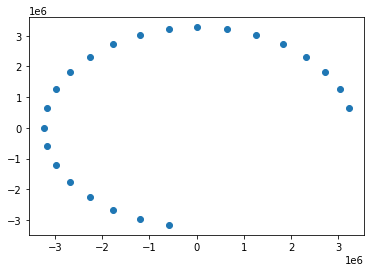
\includegraphics[width=8cm]{src/starfield/plot.png}}%
    \end{adjustbox}
  \caption{Each of the 32 points as plotted using the X/Y values calculated using the procedure above.}
\end{figure}

The remainder of the routine calculates a Z value for our point in 3D space and this one is even more
intricate.

\begin{lstlisting}[caption=Calculating the Z and color value for the starfield data structure used in the Tempest 2000 credits screen.]
  ; Calculate the Z value.
  lsl #2,d0
  and #$ff,d0
  move.b 0(a1,d0.w),d1
  move.b 0(a2,d0.w),d2
  and #$f0,d2
  lsl #4,d2
  ext d1
  bpl sposss
  neg d1
sposss:
  swap d1
  clr d1
  asr.l #1,d1
  clr.l d0
  move d7,d0
  swap d0
  lsl.l #6,d0    ;Z position according to ring no.
  add.l d1,d0
  move.l d0,(a0)+ ; Move Z into our star data structure

  move d4,d0
  add d2,d0
  move d0,(a0)    ;colour
  lea 20(a0),a0
  dbra d6,ring2
  add #$2000,d4
  dbra d7,ring1
  rts
\end{lstlisting}

